\documentclass[sans]{beamer}
%\documentclass[handout]{beamer}
%\usepackage{pst-plot}
\usepackage{tikz}
\usepackage[latin1]{inputenc}
\usepackage[T1]{fontenc}
\usepackage{times}

\theoremstyle{definition}
\theoremstyle{theorem}
\newtheorem{resultat}{Resultat}
\newtheorem{defin}{Definisjon}
\newtheorem{repi}{Repitisjon}
\title{PPU3210: Matematikkdiadaktikk\\
Annengradslikninger}
\author{Gruppe G:\\
Christian Gustad\\
Niels Bonten\\
Ola Fosheim Gr�stad\\
Tharald Stray Laastad\\
}
\date{\today}
\usetheme{Copenhagen}
\setbeamertemplate{caption}{\raggedright\insertcaption\par}
\setbeamertemplate{footline}{}
\begin{document}


\frame{\maketitle}

\begin{frame}{Grafisk l�sning}
\begin{defin}
En annnengradslikning er et utrykk p� formen:
\begin{displaymath}
a\cdot x^2 + b\cdot x + c = 0.
\end{displaymath}
\end{defin}
\begin{itemize}
\item Dette kan blandt annet relateres til kastebaner og geometriske problemer.\\
\item Grafisk dr�fning gj�r at vi enkelt kan observere tilfeller der grafen skj�rer $x$ aksen:
\end{itemize}

\begin{minipage}{.2\textwidth}
\begin{figure}
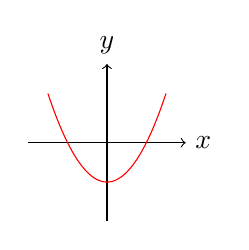
\begin{tikzpicture}
      \draw[->] (-1,0) -- (1,0) node[right] {$x$};
      \draw[->] (0,-1) -- (0,1) node[above] {$y$};
      \draw[scale=0.5,domain=-1.5:1.5,smooth,variable=\x,red] plot ({\x},{(\x-1)*(\x+1)});
\end{tikzpicture}
\caption{To l�sninger}
\end{figure}
\end{minipage}
\hfill
\begin{minipage}{.2\textwidth}
%\caption{En l�sning}
\begin{figure}
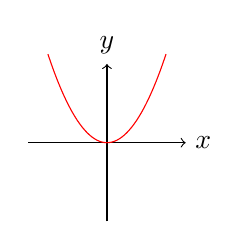
\begin{tikzpicture}
      \draw[->] (-1,0) -- (1,0) node[right] {$x$};
      \draw[->] (0,-1) -- (0,1) node[above] {$y$};
      \draw[scale=0.5,domain=-1.5:1.5,smooth,variable=\x,red] plot ({\x},{\x*\x});
\end{tikzpicture}
\caption{Unik l�sning}
\end{figure}
\end{minipage}
\hfill
\begin{minipage}{.2\textwidth}
\begin{figure}
%\caption{Ingen l�sning}
\begin{tikzpicture}      \draw[->] (-1,0) -- (1,0) node[right] {$x$};
      \draw[->] (0,-1) -- (0,1) node[above] {$y$};
      \draw[scale=0.5,domain=-1.2:1.2,smooth,variable=\x,red] plot ({\x},{(-\x*\x - 0.5)});
\end{tikzpicture}
\caption{Ingen l�sning}
\end{figure}
\end{minipage}

\end{frame}

\begin{frame}{Algebraisk l�sning}
  \begin{itemize}
  \item Vi angriper det algebraiske problemet med � l�se annengradslikninger.
  \item Vi skal benytte oss av en metode som kalles fullstedig kvadrat/ fullf�ring av kvadrat.
  \item Dette benytter seg av kvadratsetningene.
 \end{itemize}
\begin{repi}[Kvadratsetningene]
\[
(\alpha \pm \beta)^2 = \alpha^2 \pm2\alpha\beta+\beta^2
\]
\end{repi}
\end{frame}


\begin{frame}{Eksempel p� fullf�ring av kvadrat:}
  \begin{align*}
    x^2 + 2x - 8 & = 0 \\
    x^2 + 2x & = 8 \\
  \end{align*}
Legg til en p� begge sider:
\begin{align*}
  x^2 + 2x + 1 = 9
\end{align*}
Ved hjelp av f�rste-kvadratsetning ser vi at for $\alpha = x, \beta = 1$ har vi at:
\begin{align*}
  \left( x+1 \right)^2 = 9 
\end{align*}
Trekk s� roten p� begge sider og flytt over:
\begin{align*}
  x + 1 & = \pm 3\\
  x & = \pm 3 -1
\end{align*}
\end{frame}

\begin{frame}{$abc$-formelen}
  \begin{itemize}
  \item Dette gir elevene en metode � l�se likninger p�.
  \item Dette motiverer og illustrerer hvordan $abc$-formelen utledes.
  \item Deretter vil elevene arbeide med hvordan man l�ser andregradslikninger ved hjelp av $abc$-formelen
  \end{itemize}
  \begin{resultat}
    For ett gitt annengradsutrykk
\[
a \cdot x^2 + b\cdot x + c = 0
\]
Vil l�sningen kunne utrykkes som
\[
x = \frac{-b \pm \sqrt{b^2 -4ac}}{2a}
\]
  \end{resultat}
\end{frame}
\begin{frame}{Konklusjon}
  \begin{itemize}
  \item Den grafiske tolkningen av annengradslikninger gir ett enkelt bilde av hva det vil si � l�se en slik likning og hvordan: flere,unik og ingen l�sning kan oppst�. 
  \item Dette gj�r det at det blir lett � relatere paraboler til kasterbaner. 
  \item Vi gj�r dette for � illustrere at $abc$-formelen ikke er en magisk formel men at det finns ett system bak det.
  \item Disse metodene styrker elevenes forst�else av koblingen mellom grafer og algebra, samnt f�r repetert og sett nytten av kvadratsetningene.
  \end{itemize}
\end{frame}
\end{document}




